\documentclass[xcolor=dvipsnames]{beamer}
  \usepackage{eso-pic}
  \usepackage{lmodern}% http://ctan.org/pkg/lm
  \usepackage{fix-cm} % Fixes warnings about missing fonts; see http://tex.stackexchange.com/questions/32378/xfrac-siunitx-gives-me-a-font-warning
  \usepackage{stmaryrd}
  \usepackage{soul}
  \usepackage{amssymb,amsthm,amsmath,amsxtra}
  \usepackage[all]{xy}
  \usepackage{xfrac}
  \usepackage{calc}
  \usepackage{tikz}
  \usetikzlibrary{arrows,calc,automata,shadows,backgrounds,positioning,intersections,fadings,decorations.pathreplacing,shapes,snakes, matrix}
  \usepackage{tikz-cd}
  \tikzset{commutative diagrams/.cd, arrow style = tikz, diagrams = {>=latex}}
  \tikzset{>=latex}
  \usepackage{marvosym}
  \usepackage[marvosym]{tikzsymbols}
  \usepackage{beamerthemesplit}
  \usecolortheme[named=SeaGreen]{structure}
  % \usetheme{Singapore}
  % \setbeamersize{text margin top=-1in}
  \setbeamertemplate{navigation symbols}{}%remove navigation symbols
  \addtolength{\parskip}{0.5\baselineskip}
  \setlength{\arraycolsep}{2pt}
  \DeclareMathOperator{\area}{area}
  \DeclareMathOperator{\opchar}{char}
  \DeclareMathOperator{\opdiv}{div}
  \DeclareMathOperator{\grad}{grad}
  \DeclareMathOperator{\Cl}{Cl}
  \DeclareMathOperator{\disc}{disc}
  \DeclareMathOperator{\Gal}{Gal}
  \DeclareMathOperator{\id}{id}
  \DeclareMathOperator{\M}{M}
  \DeclareMathOperator{\tr}{tr}
  \DeclareMathOperator{\nrd}{nrd}
  \DeclareMathOperator{\opP}{P}
  \DeclareMathOperator{\OO}{O}
  \DeclareMathOperator{\PGL}{PGL}
  \DeclareMathOperator{\GL}{GL}
  \DeclareMathOperator{\PSL}{PSL}
  \DeclareMathOperator{\PSU}{PSU}
  \DeclareMathOperator{\SL}{SL}
  \DeclareMathOperator{\SO}{SO}
  \DeclareMathOperator{\vol}{vol}
  \DeclareMathOperator{\rad}{rad}
  \newcommand{\quat}[2]{\displaystyle{\bigly(\frac{#1}{#2}\biggr)}}
  \theoremstyle{plain}
  \newtheorem*{thm}{Theorem}
  \newtheorem*{ques}{Question}
  \newcommand{\psmod}[1]{~(\textup{\text{mod}}~{#1})}
  \newcommand{\C}{\mathbb C}
  \newcommand{\CC}{\mathbb C}
  \newcommand{\F}{\mathbb F}
  \newcommand{\HH}{\mathbb H}
  \newcommand{\PP}{\mathbb P}
  \newcommand{\R}{\mathbb R}
  \newcommand{\Q}{\mathbb Q}
  \newcommand{\Z}{\mathbb Z}
  \newcommand{\Qbar}{\overline{\mathbb Q}}
  \newcommand{\calD}{\mathcal{D}}
  \newcommand{\calG}{\mathcal{G}}
  \newcommand{\calH}{\mathcal H}
  \newcommand{\calO}{\mathcal O}
  \usepackage{booktabs}
  \newcommand{\defi}[1]{\textbf{#1}} 				% for defined terms
  \setlength{\hfuzz}{4pt}
  \newcommand{\Belyi}{Bely\u{\i}}
  \newcommand{\legen}[2]{\left(\frac{#1}{#2}\right)}

\title{$2$-Solvable \Belyi Maps}
\author{Michael Musty}
\date{}

\newcommand\AtPagemyUpperLeft[1]{\AtPageLowerLeft{%
\put(\LenToUnit{0.87\paperwidth},\LenToUnit{0.815\paperheight}){#1}}}
\newcommand\AtPagemyLowerRight[1]{\AtPageLowerLeft{%
  \put(\LenToUnit{0.88\paperwidth},\LenToUnit{0.02\paperheight}){#1}}}
\AddToShipoutPictureFG{
  \AtPagemyUpperLeft{{
\includegraphics[scale=.081]{chseal-white.png}}}
  \AtPagemyLowerRight{
    \usebeamerfont{framenumber}\insertframenumber{} / \inserttotalframenumber\hspace*{2ex}
  }
}%

\begin{document}
  \begin{frame}[plain]
    \begin{center}{
      \Huge\color{SeaGreen}
      $2$-solvable
      \Belyi\ maps
    }
    \end{center}
    \begin{center}
      %\includegraphics[scale = .3]{4A.pdf}
      %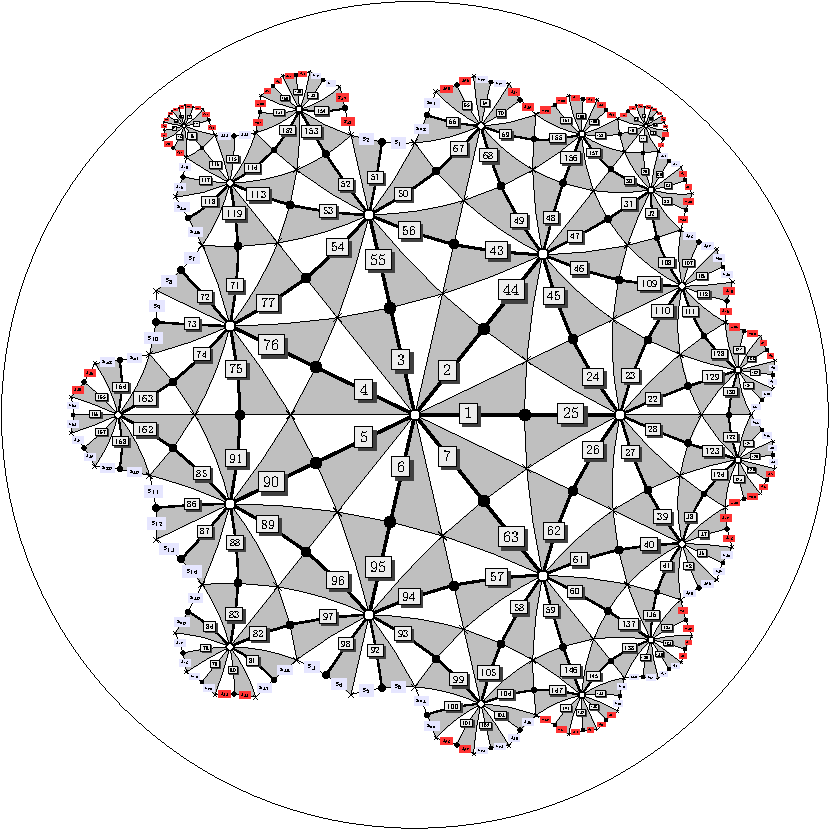
\includegraphics[scale = .3]{168A.pdf}
      %\includegraphics[scale = 0.3]{168Abw.pdf}
      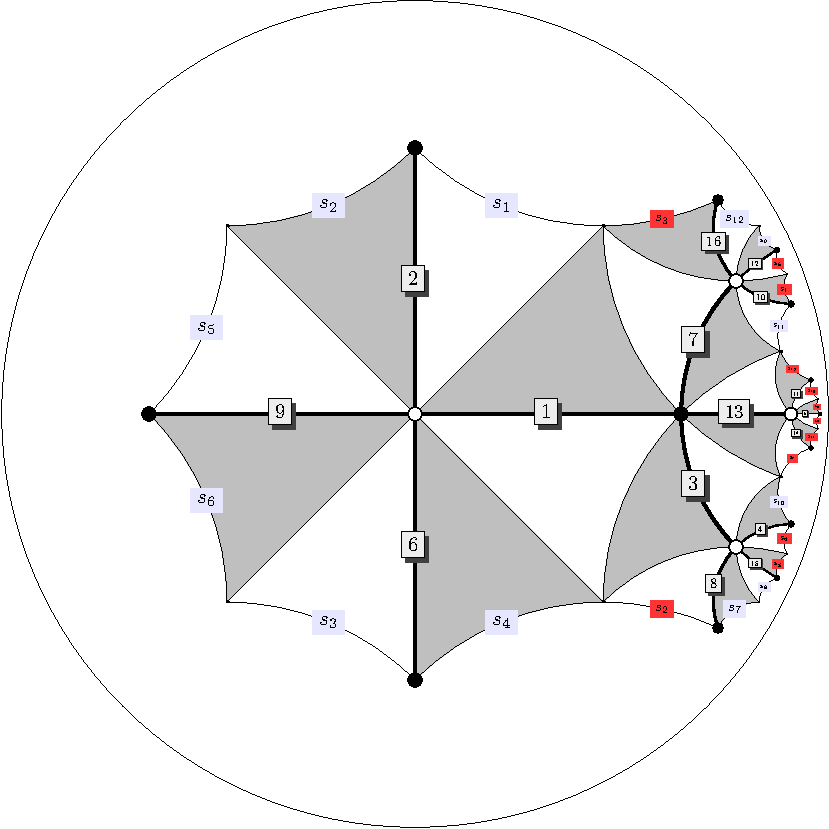
\includegraphics[scale = 0.3]{16T8-g3.pdf}
    \end{center}
    \begin{center}
      Michael Musty\\
      Algebra and Number Theory Seminar\\
      May 8, 2018
    \end{center}
  \end{frame}
  \begin{frame}[plain]
    \frametitle{Outline}
    \begin{enumerate}
      \item
        What is a 2-solvable \Belyi\ map?
      \item
        Motivation
      \item
        Algorithm to compute explicitly
        \begin{enumerate}
          \item
            Find permutation triples
          \item
            Compute equations
        \end{enumerate}
      \item
        Explicit examples
    \end{enumerate}
  \end{frame}
  \begin{frame}[plain]
    \frametitle{\Belyi's Theorem}
    \pause
    \begin{thm}[G.V. \Belyi\ 1979]
      A smooth projective curve $X$ over $\C$
      can be defined over $\overline{\Q}$ if and only if there
      exists a branched covering of compact connected Riemann surfaces $\varphi:X\to\PP^1$
      unramified (unbranched) above $\PP^1\setminus\{0,1,\infty\}$.
    \end{thm}
    \pause
    Such a map is called a \textbf{\Belyi\ map}.
    \pause
    \newline
    \newline
    In the 1980s,
    Grothendieck described a bijection
    between \Belyi\ maps and \emph{dessins d'enfants}.
    \pause
    $\Gal(\overline{\Q}/\Q)$ acts on these sets.
  \end{frame}
  \begin{frame}[plain]
    \frametitle{A Zoo of Bijections}
    \pause
    \begin{center}
      \begin{tikzpicture}[scale=.7]
        \node at (0,0) (dessins)
        {
          $
            \left\{
              \begin{minipage}{11ex}
                dessins with $d$ edges
              \end{minipage}
            \right\}
          $
        };
        \node at (-5,3) (perms)
        {
          $
            \left\{
              \begin{minipage}{22ex}
                Transitive permutation Triples
                $(\sigma_0,\sigma_1,\sigma_\infty)\in S_d^3$
                with $\sigma_\infty\sigma_1\sigma_0 = 1$
              \end{minipage}
            \right\}
          $
        };
        \node at (5,3) (triangles)
        {
          $
            \left\{
              \begin{minipage}{22ex}
                Index $d$ triangle subgroups
                $\Gamma \leq \Delta(a,b,c)$
              \end{minipage}
            \right\}
          $
        };
        \node at (5,-3) (belyis)
        {
          $
            \left\{
              \begin{minipage}{22ex}
                \Belyi\ maps of degree $d$
              \end{minipage}
            \right\}
          $
        };
        \node at (-5,-3) (fields)
        {
          $
            \left\{
              \begin{minipage}{22ex}
                Degree $d$ function
                field extensions $K \supseteq \C(z)$
                with discriminant supported above $0,1,\infty$
              \end{minipage}
            \right\}
          $
        };
        \draw[<->] (dessins) to node [above,rotate=-35] {$\sim$} node {} (perms);
        \draw[<->] (dessins) to node [above,rotate=-35] {$\sim$} node {} (belyis);
        \draw[<->] (dessins) to node [above,rotate=35] {$\sim$} node {} (triangles);
        \draw[<->] (dessins) to node [above,rotate=35] {$\sim$} node {} (fields);
      \end{tikzpicture}
    \end{center}
    \pause
    All up to the appropriate version of
    equivalence in each category.
  \end{frame}
  \begin{frame}[plain]
    \frametitle{Example \Coffeecup}
    \begin{center}
      \begin{tikzpicture}[scale=.37]
        % dashed
          %\draw[blue,ultra thin,dashed] (4,10.5)--(6,15);
        \draw[gray,ultra thin,dashed] (10,13.5)--(12,18);
        \draw[<-,black,thin,dashed] (4,3)--(4,17);
        \draw[<-,black,thin,dashed] (10,3)--(10,13.5);
        % ComplexPlane
        \draw[thick] (0,0)--(14,0)--(17,6)--(3,6)--(0,0);
        % sheet 1
          %\draw[thick,red] (8,9)--(14,9)--(17,15)--(15.5,15);
        % sheet 2
        \draw[blue,thick] (6,12)--(0,12)--(1.5,15);
        \draw[blue,thick] (15.5,18)--(17,18)--(14,12);
        % sheet 3
        \draw[gray,thick] (6,15)--(0,15)--(3,21)--(17,21)--(14,15);
        % branching
          %\draw[red,thick] (0,9)--(1.5,11.5);
          %\draw[red,thick] (0,9) to[out=0,in=-180] (4,10.5);
          %\draw[red,thick] (4,10.5) to[out=0,in=-180] (8,9);
          %\draw[blue,thick] (0,12) to[out=0,in=-180] (4,10.5);
          %\draw[blue,thick] (4,10.5) to[out=0,in=-180] (10,13.5);
        \draw[blue,thick] (6,12) to[out=0,in=-180] (10,13.5);
        \draw[blue,thick] (10,13.5) to[out=0,in=-180] (14,12);
        \draw[gray,thick] (6,15) to[out=0,in=-180] (10,13.5);
        \draw[gray,thick] (10,13.5) to[out=0,in=-180] (14,15);
        % points
        \fill [black] (4,3) circle (4pt);
        \node at (4,3) [label=right:$1$] {};
        \fill [black] (10,3) circle (4pt);
        \node at (10,3) [label=right:$0$] {};
          %\fill [black] (10,11) circle (4pt);
          %\node at (12.5,11) {$x=1/2$};
        \fill [black] (4,13.5) circle (4pt);
        \node at (6,13.5) {$x_1=1$};
        \fill [black] (4,17) circle (4pt);
        \node at (6.5,17) {$x_1=-1$};
        \fill [black] (10,13.5) circle (4pt);
        \node at (13,13.5) {$x_1=0$};
        \fill [black] (7,1) circle (4pt);
        \node at (7,1) [label=right:$\infty$] {};
        % misc
          %\node[red] at (-1,9) {$1$};
        \node[blue] at (-1,12) {$1$};
        \node[gray] at (-1,15) {$2$};
        \node at (19,18.75) {$X_1$};
        \node at (19,5.25) {$X_0=\PP^1$};
        \draw[black,->] (19,18)--(19,6);
        \node at (23.5,13) {$x_0=\varphi(x_1)=x_1^2$};
        \node at (24.75,11) {$=(x_1+1)(x_1-1)+1$};
      \end{tikzpicture}
    \end{center}
    %\pause
    %\begin{align*}
    %  \pi_1\left(\PP^1\setminus\{0,1,\infty\},*\right)\cong\langle\gamma_0,\gamma_1,\gamma_\infty\mid\gamma_\infty\gamma_1\gamma_0 = 1\rangle\to S_d
    %\end{align*}
  \end{frame}
  \begin{frame}[plain]
    \frametitle{Example \Coffeecup}
    \begin{center}
      \begin{tikzpicture}[scale=.7]
        \node at (0,0) (dessins)
        {
          \begin{tikzpicture}[
              scale=1,
              node distance=1.75cm,
              vblack/.style={circle,draw=black,fill=black,thick},
              vwhite/.style={circle,draw=black,fill=white,thick}
            ]
            \node[vwhite] (A) {};
            \node[right=of A, vblack] (B) {};
            \node[left=of A, vblack] (C) {};
            \draw[thick] (A) to node [above] {$2$} node {} (B);
            \draw[thick] (A) to node [above] {$1$} node {} (C);
          \end{tikzpicture}
        };
        \node at (-5,3) (perms)
        {
          $
          \Big((1\,2), (1)(2), (1\,2)\Big)
          $
        };
        \node at (5,3) (triangles)
        {
          $
            [\Delta(2,\infty,2) : \Gamma] = 2
          $
        };
        \node at (5,-3) (belyis)
        {
          $
          x_0=\varphi(x_1) = x_1^2
          $
        };
        \node at (-5,-3) (fields)
        {
          $
          \C\left(x_1^2\right)\subseteq\C(x_1)
          $
        };
        \draw[<->] (dessins) to node [above,rotate=-35] {$\sim$} node {} (perms);
        \draw[<->] (dessins) to node [above,rotate=-35] {$\sim$} node {} (belyis);
        \draw[<->] (dessins) to node [above,rotate=35] {$\sim$} node {} (triangles);
        \draw[<->] (dessins) to node [above,rotate=35] {$\sim$} node {} (fields);
      \end{tikzpicture}
    \end{center}
  \end{frame}
  \begin{frame}[plain]
    \frametitle{$2$-solvable (Galois) \Belyi\ maps}
    %A \defi{$2$-solvable \Belyi\ map} is a (Galois)
    %\Belyi\ map whose monodromy group is a $2$-group.
    \pause
    \begin{center}
      \begin{tikzpicture}[scale=.7]
        \node at (0,0) (X0) {$X_0 = \PP^1$};
        \node [above left=of X0] (X1) {$X_1$};
        \node [above =of X1] (X2) {$X_2$};
        \node [above =of X2] (dots) {$\vdots$};
        \node [above =of dots] (Xr) {$X_r$};
        %\draw[<->] (X1) to node [above,rotate=-35] {$\sim$} node {} (X0);
        \draw[->] (X1) to node [below] {$2$} node {} (X0);
        \draw[->] (X2) to node [left] {$2$} node {} (X1);
        \draw[->, bend left] (X2) to node [below, left] {} node {} (X0);
        \draw[->] (dots) to node [left] {$2$} node {} (X2);
        \draw[->] (Xr) to node [left] {$2$} node {} (dots);
        \draw[->, bend left] (Xr) to node [below, left] {} node {} (X0);
        \node at (8,0) (KX0) {$K(X_0) = K(\PP^1)$};
        \node [above left=of KX0] (KX1) {$K(X_1)$};
        \node [above =of KX1] (KX2) {$K(X_2)$};
        \node [above =of KX2] (dots) {$\vdots$};
        \node [above =of dots] (KXr) {$K(X_r)$};
        %\draw[<->] (X1) to node [above,rotate=-35] {$\sim$} node {} (X0);
        \draw[-] (KX1) to node [below] {$2$} node {} (KX0);
        \draw[-] (KX2) to node [left] {$2$} node {} (KX1);
        \draw[-, bend left] (KX2) to node [below, left] {} node {} (KX0);
        \draw[-] (dots) to node [left] {$2$} node {} (KX2);
        \draw[-] (KXr) to node [left] {$2$} node {} (dots);
        \draw[-, bend left] (KXr) to node [below, left] {} node {} (KX0);
      \end{tikzpicture}
    \end{center}
  \end{frame}
  \begin{frame}[plain]
    \frametitle{Beckmann's Theorem}
    \pause
    \begin{thm}[Beckmann-Kazez 1989]
      Let $\varphi:X\to\PP^1$ be a \Belyi\ map with monodromy group $G$.
      \pause
      Suppose $p$ does not divide $\#G$.
      \pause
      Then there exists a number field $M$ such that $p$
      is unramified in $M$ and
      \pause
      $\varphi$ is defined over $M$ with good reduction at all
      primes $\mathfrak{p}$ of $M$ above $p$.
    \end{thm}
    \pause
    \textbf{Upshot}:
    \pause
    Every $2$-solvable \Belyi\ curve we write down has
    good reduction away from $p=2$.
  \end{frame}
  \begin{comment}
  \end{comment}
  \begin{frame}[plain]
    \frametitle{Lifting example \Coffeecup}
    \pause
    \[
      \begin{tikzcd}[ampersand replacement=\&]
        \widetilde{X}\arrow{dd}[swap]{\widetilde{\varphi}}\arrow{dr}{\psi}\\
        \&X\arrow{dl}{\varphi}\\
        \PP^1
      \end{tikzcd}
      \quad
      \begin{tikzcd}[ampersand replacement=\&]
        K(\widetilde{X})\arrow[-]{dd}[swap]{}\arrow[-]{dr}{2}\\
        \&K(X)\arrow[-]{dl}{2}\\
        K(\PP^1)
      \end{tikzcd}
      \quad
      \begin{tikzcd}[ampersand replacement=\&]
        \{1\}\arrow[-]{dd}[swap]{}\arrow[-]{dr}{2}\\
        \&H\arrow[-]{dl}{2}\\
        \widetilde{G}
      \end{tikzcd}
    \]
    \pause
    \begin{align*}
      G &= \Gal(K(X)/K(\PP^1))&&G\cong\left\langle\Big((1\,2),(1)(2),(1\,2)\Big)\right\rangle\leq S_2\\
      \widetilde{G} &= \Gal(K(\widetilde{X})/K(\PP^1))&&\widetilde{G}\cong\langle\widetilde{\sigma}\rangle\leq S_{4}\\
      H &= \Gal(K(\widetilde{X})/K(X))&&H\cong\langle(1\,3)(2\,4)\rangle\leq S_{4}
    \end{align*}
    \pause
    \[
      \begin{tikzcd}[ampersand replacement=\&, row sep = small]
        1\arrow{r}\&H\arrow{r}{\iota}\&\widetilde{G}\arrow{r}{f}\&G\arrow{r}\&1\\
        \&\&\widetilde{\sigma}\arrow{r}{?}\&\sigma
      \end{tikzcd}
    \]
  \end{frame}
  \begin{frame}[plain]
    \frametitle{Lifting example \Coffeecup}
    \pause
    \begin{align*}
      \sigma &= (\sigma_0,\sigma_1,\sigma_\infty)
      =\Big((1\,2),(1)(2),(1\,2)\Big)\in S_2^3\\
      \tau &= (1\,3)(2\,4)\in S_4\\
      \widetilde{G} &= \langle\widetilde{\sigma}\rangle\leq S_4
    \end{align*}
    \pause
    \[
      \begin{tikzcd}[ampersand replacement=\&, row sep = small]
        1\arrow{r}\&\langle\tau\rangle\arrow{r}{\iota}\&\widetilde{G}\arrow{r}{f}\&\langle\sigma\rangle\arrow{r}\&1\\
        \&\&\widetilde{\sigma}\arrow{r}{?}\&\sigma
      \end{tikzcd}
    \]
    \pause
    \begin{center}
      \begin{tabular}{ccc}
        \toprule
        $f^{-1}(\sigma_0)$
        & $f^{-1}(\sigma_1)$
        & $f^{-1}(\sigma_\infty)$\\
        \midrule
        $(1\,2)(3\,4)$ & $(1)(2)(3)(4)$ & $(1\,2)(3\,4)$\\
        $(1\,4)(2\,3)$ & $(1\,3)(2\,4)$ & $(1\,4)(2\,3)$\\
        $(1\,4\,3\,2)$ && $(1\,4\,3\,2)$\\
        $(1\,2\,3\,4)$ && $(1\,2\,3\,4)$\\
        \bottomrule
      \end{tabular}
    \end{center}
  \end{frame}
  \begin{frame}[plain]
    \frametitle{Lifting example \Coffeecup}
    \pause
    \par
    There are 32 possible $\sigma$ from these lists.
    \pause
    \par
    Only 6 such triples correspond to \Belyi\ maps.
    \pause
    \par
    3 of these triples
    corresponding to distinct \Belyi\ maps (up to isomorphism).
    \pause
    \begin{center}
      \begin{tabular}{c}
        \toprule
        $\widetilde{G}\cong\Z/4\Z$\\
        \midrule
        $\Big((1\,4\,3\,2),(1)(2)(3)(4),(1\,2\,3\,4)\Big)$\\
        $\Big((1\,4\,3\,2),(1\,3)(2\,4),(1\,4\,3\,2)\Big)$\\
        \bottomrule
      \end{tabular}
    \end{center}
    \begin{center}
      \begin{tabular}{c}
        \toprule
        $\widetilde{G}\cong\Z/2\Z\times\Z/2\Z$\\
        \midrule
        $\Big((1\,2)(3\,4),(1\,4)(2\,3),(1\,3)(2\,4)\Big)$\\
        \bottomrule
      \end{tabular}
    \end{center}
  \end{frame}
  \begin{frame}[plain]
    \frametitle{\texttt{4T1-[4,2,4]-4-22-4-g1}}
    \pause
    \[
      (\sigma_0,\sigma_1,\sigma_\infty) = \Big((1\,4\,3\,2),(1\,3)(2\,4),(1\,4\,3\,2)\Big)
    \]
    \pause
    \begin{tikzpicture}[scale=.5]
      %\draw[thin,gray] (-20,-1) grid (20,5);
      % Y1 to Y0
      % affine curves
      \node (Y0) at (0,0) {$X_0$};
      \node (Y1) at (-4,5) {$X_1:x_1^2=x_0$};
      \node (Y2) at (-4,10) {$X_2:\substack{x_1^2=x_0\\x_2^2=x_1^3-x_1}$};
      % maps of affine curves
      %\draw[->] (Y1)--(Y0) node [pos=.5,left] {$(x_0,x_1)\mapsto x_0=x_1^2$};
      \draw[->] (Y1)--(Y0);
      %\draw[->] (Y2)--(Y1) node [pos=.5,left] {$(x_0,x_1)$};
      \draw[->] (Y2)--(Y1);
      %\draw[->,thick,blue,bend left] (Y2) to node [pos=.25,right] {$x_0 = x_1^2$} (Y0);
      \draw[->,thick,bend left] (Y2) to (Y0);
      % function fields
      \node (KX0) at (20,0) {$K(X_0) = K(x_0)$};
      \node (KX1) at (16,5) {$K(X_1) = \frac{K(x_0)[x_1]}{\left(x_1^2-x_0\right)}$};
      \node (KX2) at (16,10) {$K(X_2) = \frac{K(X_1)[x_2]}{\left(x_2^2-(x_1^3-x_1)\right)}$};
      \draw[->] (KX0) to (KX1);
      \draw[->] (KX1) to (KX2);
      \draw[->,thick,blue,bend right] (KX0) to (KX2);
      % ramification
      \node (Y0 0) at (-20,0) {$0$};
      \node (Y0 1) at (-15,0) {$1$};
      \node (Y0 oo) at (-10,0) {$\infty$};
      \node (Y1 0) at (-20,5) {$(0,0)$};
      \node (Y1 1) at (-20+10/3,5) {$(1,1)$};
      \node (Y1 -1) at (-20+20/3,5) {$(1,-1)$};
      \node (Y1 oo) at (-10,5) {$\infty$};
      \node (Y2 0) at (-20,10) {$(0,0,0)$};
      \node (Y2 1) at (-20+10/3,10) {$(1,1,0)$};
      \node (Y2 -1) at (-20+20/3,10) {$(1,-1,0)$};
      \node (Y2 oo) at (-10,10) {$\infty$};
      \draw[double distance=1pt] (Y1 0) to (Y0 0);
      \draw (Y0 1) to (Y1 1);
      \draw (Y1 -1) to (Y0 1);
      \draw[double distance=1pt] (Y1 oo) to (Y0 oo);
      \draw[double distance=1pt] (Y2 0) to (Y1 0);
      \draw[double distance=1pt] (Y2 1) to (Y1 1);
      \draw[double distance=1pt] (Y2 -1) to (Y1 -1);
      \draw[double distance=1pt] (Y2 oo) to (Y1 oo);
    \end{tikzpicture}
  \end{frame}
  \begin{frame}[plain]
    \frametitle{\texttt{16T6-[8,8,4]-88-88-4444-g5}}
    \pause
    We now exhibit a genus $5$ \Belyi\ map $\varphi:X\to\PP^1$ defined by $x_0\in K(X)$
    with monodromy group $C_8:C_2$.
    \pause
    \par
    $X$ is cut out by the following equations in $\mathbb{A}^5$:
    \pause
    \begin{align*}
      x_1^2 &= x_0\\
      x_3x_4^2 &= x_1x_2+x_1+x_3^2\\
      x_3x_4^2 &= x_1+x_1x_3^2\\
      x_3x_4^4 &= x_3^3+2x_1x_4^2\\
      2x_3^2x_4^4 &= x_2^2+2x_3^3x_4^2+2x_3^2-2x_3x_4^2+2x_4^4+1\\
      x_3^3 &= x_2x_3+x_3^2x_4^2-x_4^2\\
      x_3^2x_4^2 &= x_2x_4^2+x_3^3+x_3\\
      x_3^2x_4^4 &= x_3^4+x_3^2+x_4^4
    \end{align*}
  \end{frame}
  \begin{frame}[plain]
    \frametitle{Acknowledgements}
    Thanks to the following for helpful discussions:
    \begin{itemize}
      \item Sam Schiavone
      \item Jeroen Sijsling
      \item John Voight
    \end{itemize}
  \end{frame}
  \begin{frame}[plain]
    \frametitle{Thanks for listening!}
    \url{https://math.dartmouth.edu/~mjmusty/32.html}
  \end{frame}
\end{document}
